\documentclass[UTF8,zihao=-4,fontset=fandol]{ctexart}

\usepackage[a4paper,top=2.5cm,bottom=2.5cm,left=2.7cm,right=2.7cm]{geometry}
\usepackage{amsmath,amssymb}
\usepackage{booktabs,longtable,tabularx,array,multirow}
\usepackage{graphicx,float}
\usepackage{xcolor}
\usepackage{tikz}
\usetikzlibrary{arrows.meta,positioning,fit,calc,shapes.geometric}
\usepackage{pgfplots}
\pgfplotsset{compat=1.18}
\usepackage{listings}
\usepackage{enumitem}
\usepackage{caption}
\usepackage{fancyhdr}
\usepackage{xurl}
\usepackage{hyperref}
\usepackage[backend=biber,style=numeric,sorting=none]{biblatex}
\addbibresource{references.bib}

\setmainfont[
  Path=/usr/local/texlive/2026/texmf-dist/fonts/opentype/public/stix2-otf/,
  BoldFont=STIXTwoText-Bold.otf,
  ItalicFont=STIXTwoText-Italic.otf,
  BoldItalicFont=STIXTwoText-BoldItalic.otf
]{STIXTwoText-Regular.otf}
\AtBeginBibliography{\sloppy}

\definecolor{zetablue}{HTML}{2563EB}
\definecolor{zetacyan}{HTML}{0891B2}
\definecolor{zetagreen}{HTML}{059669}
\definecolor{zetaorange}{HTML}{D97706}
\definecolor{zetared}{HTML}{DC2626}
\definecolor{zetagray}{HTML}{475569}
\definecolor{zetalight}{HTML}{F1F5F9}

\hypersetup{
  colorlinks=true,
  linkcolor=zetablue,
  citecolor=zetagreen,
  urlcolor=zetacyan,
  pdftitle={zeta-engine：面向中文高校网站的混合检索与证据约束 RAG 引擎设计与实现},
  pdfauthor={zeta-engine 项目组}
}

\pagestyle{fancy}
\fancyhf{}
\fancyhead[L]{\small ζ-engine 技术报告}
\fancyhead[R]{\small 混合检索与证据约束 RAG}
\fancyfoot[C]{\thepage}
\setlength{\headheight}{14pt}

\setlength{\parindent}{2em}
\setlength{\parskip}{0.25em}
\linespread{1.35}
\setlist{nosep,leftmargin=2em}
\captionsetup{font=small,labelfont=bf}
\renewcommand{\arraystretch}{1.22}

\lstset{
  basicstyle=\ttfamily\small,
  backgroundcolor=\color{zetalight},
  frame=single,
  rulecolor=\color{zetagray!35},
  breaklines=true,
  columns=fullflexible,
  keepspaces=true,
  showstringspaces=false,
  keywordstyle=\color{zetablue}\bfseries,
  commentstyle=\color{zetagreen},
  stringstyle=\color{zetaorange},
  numbers=left,
  numberstyle=\tiny\color{zetagray},
  xleftmargin=2em,
  framexleftmargin=1.5em
}

\newcommand{\project}{ζ-engine}
\newcommand{\passage}{Passage}
\newcommand{\code}[1]{\texttt{#1}}
\newcommand{\keywords}[1]{\par\noindent\textbf{关键词：}#1}

\title{\bfseries\Huge ζ-engine\par\vspace{0.5em}
  \LARGE 面向中文高校网站的混合检索与证据约束 RAG 引擎设计与实现}
\author{zeta-engine 项目组\\[0.5em]\large 综合程序设计技术报告}
\date{2026 年 9 月}

\begin{document}

\maketitle
\thispagestyle{empty}
\vfill
\begin{center}
\begin{minipage}{0.82\textwidth}
\small
\textbf{项目定位：}面向中国人民大学相关站点的本地中文搜索与检索增强生成系统。\\
\textbf{技术关键词：}网页抓取；BM25F；稠密检索；混合召回；CrossEncoder；Agentic RAG；证据审计。
\end{minipage}
\end{center}
\vfill
\clearpage

\begin{abstract}
\project{} 为中国人民大学相关站点提供本地搜索与问答。按学院名称或年份查找通知时，用户需要准确定位网页；询问政策、办事流程或名单人数时，还需要从网页中整理答案。项目据此实现了词法与语义混合检索，并为问答保留可追溯的原文证据。

爬虫将网页正文保存为纯文本和最小语义 HTML。前者用于索引，后者保留表格与列表结构。文档搜索以 BM25F 为基础；RAG 将正文切成共享分块，融合稀疏与稠密检索结果，再用 CrossEncoder 重排。命中分块用于定位原文，问答时再恢复附近的表格、列表和章节。需要统计或比较完整名单时，Agent 可进一步扫描表格并调用计算工具。Verifier 检查答案是否满足提问要求、断言是否有证据支持，程序限制循环轮数与模型调用次数。

在已有的 72 条高置信查询记录中，Hybrid 取 $\alpha=0.38$ 时，MRR@20 从 BM25F 的 0.4420 升至 0.4726，相对提高约 6.9\%；Top-1 命中数由 25 增至 26，Recall@20 均为 0.7361。这组结果体现了排序改善。问答结果另附引用和计算来源，供使用者核对。

\keywords{中文搜索引擎；BM25F；稠密检索；混合检索；检索增强生成；Agent；证据溯源}
\end{abstract}

\clearpage
\tableofcontents
\clearpage

\section{引言}

\subsection{问题与设计出发点}

在高校网站上查一份通知，通常可以从学院名称、年份或通知编号入手。询问“经济困难学生如何申请资助”则不同：网页未必使用提问中的措辞，答案也可能分散在几段政策说明里。\project{} 面向中国人民大学相关站点，将这两类需求放在同一个入口中处理。查询中的专名和编号用词法匹配，自然语言问题则结合语义检索处理。

问答采用检索增强生成（Retrieval-Augmented Generation, RAG），把检索到的网页内容作为语言模型的作答依据\cite{lewis2020rag}。不过，相关段落未必包含回答所需的全部信息。一张名单表格被切成几个窗口后，单个窗口可能包含与问题相关的条目，却没有列全名单，无法据此计算总人数。为此，采集时保留网页结构，检索后再从命中位置恢复表格或章节。若计算需要完整名单，则另行扫描表格。

学校门户、学院主页和专题站点使用不同模板。提取正文时，需要去掉导航等公共内容，同时保留标题层级和表格行列关系。下文按采集、检索、证据处理和问答的顺序说明实现。

\subsection{技术目标}

\begin{enumerate}
  \item 在允许域名内并发采集，失败后重试，进程重启后恢复任务，并按策略刷新页面；
  \item 适配不同站点模板，去除公共噪声，保留表格、列表及标题层级；
  \item 同时利用专名、编号的词法匹配和同义表达的语义匹配，控制在线检索开销；
  \item 为答案断言保存证据引用，为计数、比例及集合运算保存操作数来源。
\end{enumerate}

\section{需求分析与总体架构}

\subsection{功能需求}

系统需要完成表\ref{tab:functional-requirements}中的任务。其中，搜索返回网页，RAG 返回有来源引用的答案；两者共用采集结果和索引。

\begin{table}[H]
\centering
\caption{系统主要功能需求}
\label{tab:functional-requirements}
\begin{tabularx}{\textwidth}{>{\bfseries}p{2.5cm}X X}
\toprule
模块 & 输入与处理 & 输出 \\
\midrule
网页采集 & 种子 URL、允许域名、并发数和刷新策略 & 清理后的文档、任务状态与日志 \\
索引构建 & 文档纯文本、标题、抓取版本 & 文档倒排索引、Passage FTS5、向量矩阵与元数据 \\
普通搜索 & 查询、排名模式、返回数量和融合系数 & 按相关性排序的文档、摘要和 URL \\
RAG 问答 & 自然语言问题、循环预算和模型配置 & 答案、状态、要求账本、断言、来源与调试轨迹 \\
接口服务 & CLI 参数或 HTTP 查询参数 & 终端输出、JSON 响应或 Web 页面 \\
评测 & 查询集、相关 URL 或参考答案 & MRR、召回、逐题得分和延迟 \\
\bottomrule
\end{tabularx}
\end{table}

\subsection{非功能需求}

项目按单机部署设计，程序将文档和任务状态保存在 SQLite 中，将向量索引保存为本地文件。爬虫只访问允许域名。索引构建程序通过原子操作发布新版本，避免服务读到尚未写完的索引。问答程序还限制模型调用次数和上下文规模，控制补检开销。

多轮问答会反复引用同一段内容，因此证据需要稳定 ID。应用服务以统一结构返回答案、来源和处理状态，CLI 与 HTTP 服务据此展示结果。

\subsection{总体架构}

当前代码分为七个包，图\ref{fig:q1-architecture}展示了主要调用关系。\path{interfaces} 接收在线请求，\path{application/service.py} 决定如何取得搜索结果，或准备证据后启动问答。\path{retrieval} 负责查找和恢复网页内容；\path{rag} 负责根据已有证据选择工具、生成答案并审查。

应用服务将检索和完整表格扫描封装成回调，传给 RAG 引擎；引擎调用这些工具即可取得证据，不需要依赖应用服务的实现。程序在本地完成向量编码和重排，通过 OpenAI-compatible API 调用生成模型。

CLI 直接调用 \path{ingestion}、\path{retrieval} 和 \path{evaluation}，分别执行采集、建索引和评测。\path{infrastructure} 提供共用的 SQLite 访问、文本处理和配置。

\begin{figure}[H]
\centering
\begin{tikzpicture}[
  box/.style={draw=zetablue,rounded corners,align=center,font=\small,minimum height=12mm,fill=zetablue!6},
  arrow/.style={-{Latex[length=2mm]},thick,draw=zetagray},
  note/.style={font=\scriptsize,align=center,fill=white,inner sep=2pt}
]
\node[box,text width=8.5cm] (interfaces) at (-1,0) {\texttt{interfaces}\quad CLI / HTTP\\解析请求与展示结果};
\node[box,text width=7cm] (application) at (-2,-2) {\texttt{application/service.py}\\组织搜索、证据获取与问答};
\node[box,text width=3.6cm,minimum height=19mm,fill=zetacyan!7] (retrieval) at (-4.15,-4.4) {\texttt{retrieval}\\召回、重排\\\texttt{acquisition} 获取证据};
\node[box,text width=3.6cm,minimum height=19mm,fill=zetagreen!7] (rag) at (0.15,-4.4) {\texttt{rag}\\Agent、工具、Verifier\\证据池与计算};
\node[box,text width=8.5cm,fill=zetalight] (infra) at (-2,-6.9) {\texttt{infrastructure}\\SQLite、文本处理与共享常量};
\node[box,text width=3.4cm,minimum height=33mm,fill=zetaorange!7,draw=zetaorange] (offline) at (4.8,-3.1) {CLI 直接调度\\[3pt]\texttt{ingestion}：采集\\\texttt{retrieval}：建库\\\texttt{evaluation}：评测};
\draw[arrow] (interfaces.south) -- (application.north);
\draw[arrow] (application.south west) -- node[note,left]{检索与结构恢复} (retrieval.north);
\draw[arrow] (application.south east) -- node[note,right]{注入工具回调} (rag.north);
\draw[arrow] (retrieval.south) -- (retrieval.south |- infra.north);
\draw[arrow] (rag.south) -- (rag.south |- infra.north);
\draw[arrow] (interfaces.east) -| node[note,pos=0.65,right]{离线命令} (offline.north);
\draw[arrow] (offline.south) |- (infra.east);
\node[note,text width=12.8cm] (legend) at (0,-8.2) {箭头表示主要调用方向。评测复用应用服务与检索；RAG 通过回调使用检索工具。};
\end{tikzpicture}
\caption{职责包与主要调用关系}
\label{fig:q1-architecture}
\end{figure}

\subsection{各模块的输入、处理与输出}

下面用七组流程公式概括各包的职责。箭头表示处理步骤，$q$ 为用户查询，$\tilde q$ 为规范化后的查询，$\mathcal D$ 为文档库，$E$ 为证据池。

\subsubsection*{接口层：解析请求并输出结果}

\begin{equation}
r_{\mathrm{CLI/HTTP}}
\xrightarrow{\mathrm{Parse}}(o,\theta)
\xrightarrow{\mathrm{Dispatch}}y
\xrightarrow{\mathrm{Format}}r_{\mathrm{out}}.
\label{eq:architecture-interfaces}
\end{equation}

\path{interfaces} 从请求中解析操作 $o$ 和参数 $\theta$，将搜索与问答交给应用服务，将采集、建库和评测交给对应模块。取得结果 $y$ 后，接口层将其格式化为终端文本、JSON 或 Web 页面。

\subsubsection*{应用层：组织搜索与问答}

\begin{equation}
\begin{aligned}
(q,m)&\xrightarrow{\mathrm{Normalize}}(\tilde q,m),\\
\mathrm{Service}(\tilde q,m)&=
\begin{cases}
\mathrm{SearchDocuments}(\tilde q),&m=\mathrm{search},\\
\mathrm{RAG}(\tilde q;f_s,f_c),&m=\mathrm{rag}.
\end{cases}
\end{aligned}
\label{eq:architecture-application}
\end{equation}

模式 $m$ 决定返回文档还是生成答案。\path{application} 为 RAG 构造检索回调 $f_s$ 和完整表格扫描回调 $f_c$，引擎通过这两个回调取得证据。

\subsubsection*{采集层：从网页取得正文}

\begin{equation}
\begin{aligned}
U_{\mathrm{seed}}
&\xrightarrow{\mathrm{NormalizeURL+ScopeCheck}}Q
\xrightarrow{\mathrm{Schedule+Fetch}}H,\\
H&\xrightarrow{\mathrm{Extract+Clean}}\mathcal D,\\
d&=(\mathrm{URL},\mathrm{title},\mathrm{text},h_{\mathrm{sem}}),\quad d\in\mathcal D.
\end{aligned}
\label{eq:architecture-ingestion}
\end{equation}

\path{ingestion} 从种子 URL 集合 $U_{\mathrm{seed}}$ 建立持久化队列 $Q$，下载 HTML 页面 $H$，再提取并清洗正文。文档 $d$ 同时保留纯文本和语义 HTML $h_{\mathrm{sem}}$。爬虫将新发现的合法链接加入队列，继续抓取。

\subsubsection*{检索层：建索引、排序并恢复证据}

\begin{equation}
\begin{aligned}
\mathcal D&\xrightarrow{\mathrm{Index+Chunk+Encode}}
(I_{\mathrm{BM25F}},I_{\mathrm{FTS5}},V),\\
\tilde q&\xrightarrow{\mathrm{Sparse}\,\cup\,\mathrm{Dense}}C
\xrightarrow{(1-\alpha)\tilde s_s+\alpha\tilde s_d}C'
\xrightarrow{\mathrm{CrossEncoder}}R_k,\\
R_k&\xrightarrow{\mathrm{Output}}
\begin{cases}
\mathrm{DocumentCards}(R_k),&\mathrm{search},\\
\mathrm{RecoverStructure}(R_k,\mathcal D),&\mathrm{rag}.
\end{cases}
\end{aligned}
\label{eq:architecture-retrieval}
\end{equation}

\path{retrieval} 建立文档倒排索引 $I_{\mathrm{BM25F}}$、分块索引 $I_{\mathrm{FTS5}}$ 和向量矩阵 $V$。上式表示启用混合召回与重排时的流程：程序合并两路候选得到 $C$，以归一化后的稀疏分数 $\tilde s_s$ 和稠密分数 $\tilde s_d$ 融合排序，再重排得到 $R_k$。普通搜索按文档融合分数，返回标题、URL、摘要和日期；RAG 按分块融合分数，再从原文恢复证据。

\subsubsection*{问答层：调用工具、积累证据并审查答案}

\begin{equation}
\begin{aligned}
S_0&=(\tilde q,E_0=\varnothing,L_0=\varnothing),\\
a_t&=\mathrm{Agent}(S_t),\\
S_{t+1}&=
\begin{cases}
\mathrm{Update}(S_t,\mathrm{Tool}(a_t)),&a_t\in\mathcal T,\\
\mathrm{Update}(S_t,\mathrm{Verifier}(A_t,E_t)),&a_t=\mathrm{Answer},
\end{cases}\\
S_T&\xrightarrow{\mathrm{Finalize}}(\mathrm{Answer},\mathrm{Sources},\mathrm{Status}),\\
\mathcal T&=\{\mathrm{Search},\mathrm{Collect},\mathrm{Calculate}\}.
\end{aligned}
\label{eq:architecture-rag}
\end{equation}

$S_t$ 概括第 $t$ 轮的运行状态，其中包括待处理查询、证据池 $E_t$、计算结果，以及记录要求完成情况和审查反馈的 $L_t$。Agent 选择动作 $a_t$，工具据此更新查询、证据或计算结果；提交候选答案 $A_t$ 时，Verifier 检查回答要求和证据支持情况。引擎根据反馈继续处理，或在结束时返回答案、来源和状态。默认最多运行 5 轮、调用模型 12 次，模型调用超限时引擎报错终止。

\subsubsection*{基础设施层：规范文本并持久化数据}

\begin{equation}
\begin{aligned}
x&\xrightarrow{\mathrm{NFKC+Casefold+Whitespace}}\tilde x
\xrightarrow{\mathrm{Tokenize}}\{(w_i,p_i)\},\\
B_t&\xrightarrow{\mathrm{Write}(\Delta)}B_{t+1},
\qquad(B_t,k)\xrightarrow{\mathrm{Read}}v_k.
\end{aligned}
\label{eq:architecture-infrastructure}
\end{equation}

\path{infrastructure} 将文本 $x$ 规范化后分词，得到词项 $w_i$ 及其字符位置 $p_i$。数据库访问模块把更新 $\Delta$ 写入 SQLite，使数据库状态从 $B_t$ 变为 $B_{t+1}$；读取时按查询条件 $k$ 返回记录 $v_k$。文档、任务状态和倒排记录分别保存在对应数据库中，共享常量为上层模块提供配置。

\subsubsection*{评测层：运行查询并汇总评分}

\begin{equation}
\begin{aligned}
\{q_i\}_{i=1}^{N}
&\xrightarrow{\mathrm{Search/RAG}}\{y_i\}_{i=1}^{N}
\xrightarrow{\mathrm{Submit+Score}}
\{s_i,\ell_i\}_{i=1}^{N},\\
\{s_i,\ell_i\}_{i=1}^{N}
&\xrightarrow{\mathrm{Aggregate}}\mathrm{EvaluationReport}.
\end{aligned}
\label{eq:architecture-evaluation}
\end{equation}

\path{evaluation} 调用搜索或问答服务取得结果 $y_i$，向评测服务提交答案，并汇总评分 $s_i$ 与延迟 $\ell_i$。搜索评测使用 MRR、Recall 和 Top-1 等指标，问答评测记录逐题得分与延迟。

\section{网页采集与语义正文处理}

\subsection{抓取范围与 URL 规范化}

爬虫从种子 URL 出发，为发现的链接建立抓取任务。建立任务前，程序先去掉 URL 中的片段标识（fragment），避免同一页面因锚点不同而被重复抓取。

爬虫只访问指定域名内的 HTTP/HTTPS 页面。程序在调度时、请求发出前和重定向完成后校验 URL 与主机，收到非 HTML 响应则直接跳过。

\subsection{持久化任务状态机}

\path{ingestion/crawler.py} 通过 \path{infrastructure/storage.py} 保存抓取任务。每个 URL 对应四种状态之一：\code{pending} 表示等待处理，\code{processing} 表示正在处理，\code{done} 表示已完成，\code{failed} 表示重试达到上限。

程序领取任务时增加尝试次数。抓取失败且尝试次数未达上限时，程序将任务重新加入队列；进程重启后，程序也将中断前仍在处理的任务恢复为待调度状态。已完成任务可按时间刷新，失败任务可显式重试，状态转换见图\ref{fig:crawl-state}。

\begin{figure}[H]
\centering
\begin{tikzpicture}[
  state/.style={draw=zetablue,rounded corners,minimum width=25mm,minimum height=10mm,align=center,font=\small,fill=zetablue!6},
  arrow/.style={-{Latex[length=2mm]},thick,draw=zetagray},
  note/.style={font=\scriptsize,fill=white,inner sep=2pt,align=center}
]
\node[state] (pending) at (-4,0) {pending};
\node[state,fill=zetacyan!8] (processing) at (0,0) {processing};
\node[state,draw=zetagreen,fill=zetagreen!8] (done) at (4,0) {done};
\node[state,draw=zetared,fill=zetared!6] (failed) at (0,-2.1) {failed};
\draw[arrow] (pending) -- node[note,above]{领取任务} (processing);
\draw[arrow] (processing) -- node[note,above]{保存成功或跳过} (done);
\draw[arrow] (processing.north) -- (0,1.3) -- node[note,above]{失败未超限 / 重启恢复} (-4,1.3) -- (pending.north);
\draw[arrow] (done.north) -- (4,2.5) -- node[note,above]{到期刷新} (-4,2.5) -- (-4,1.3);
\draw[arrow] (processing.south) -- node[note,right]{失败达到上限} (failed.north);
\draw[arrow] (failed.west) -- node[note,below]{显式重试} (-4,-2.1) -- (pending.south);
\end{tikzpicture}
\caption{持久化抓取任务状态机}
\label{fig:crawl-state}
\end{figure}

下载线程从内存请求队列领取任务，再把响应放入有界处理队列。协调循环负责解析页面、保存文档、发现新链接，并提交任务状态。若下载快于处理，队列填满后，下载线程就等待空位。协调循环保存文档后，将对应任务标记为 \code{done}；对于因域名或内容类型而跳过的任务，也将其标记为完成。

爬虫按目标主机限制请求频率。访问同一主机的下载线程共用下一次允许请求的时间，增加线程数不会绕过这一限制。

\subsection{正文提取规则}

教师详情、视频详情和新闻列表的正文位置不同，需要分别配置提取规则。\path{ingestion/extraction_rules.py} 用 URL 路径的正则表达式识别这类页面，依次尝试页面族规则、站点默认规则和全局规则，选出标题与正文容器，并去掉局部噪声。

爬虫优先用 BeautifulSoup 提取正文，以保留 DOM 结构；提取不到时再使用 Resiliparse。爬虫只采用其中一种提取结果，避免拼接造成内容重复或顺序混乱。

\subsection{纯文本与语义 HTML 双表示}

索引用纯文本匹配内容，问答还需要原文的结构信息。因此，爬虫将正文保存为纯文本和语义 HTML：\code{text} 存纯文本，用于分词、向量编码和摘要；\code{content\_html} 存语义 HTML，保留表格行列关系和列表层级，供问答时恢复原文结构。

清洗后的 HTML 包含标题、段落、列表、表格，也可包含引用、代码、链接和图片替代文本。清洗程序移除全部脚本、样式、表单、iframe 和 SVG；对于其他不在白名单中的普通标签，只去掉标签、保留文字。

\section{存储、规范化与稀疏检索}

\subsection{SQLite 存储设计}

存储模块用规范化 URL 唯一标识文档，刷新时通过 UPSERT 替换正文，保留原有文档 ID。\path{infrastructure/storage.py} 分别访问文档库、抓取队列库和倒排索引库，各库保存的内容见表\ref{tab:databases}。

更新倒排索引时，程序在同一事务内删除旧 posting、写入新快照与 posting，再重算受影响词项的文档频率。读取端由此不会看到只更新了一部分的索引。

\begin{table}[H]
\centering
\caption{SQLite 数据库及主要职责}
\label{tab:databases}
\begin{tabularx}{\textwidth}{>{\raggedright\arraybackslash}p{3.2cm}>{\raggedright\arraybackslash}p{4.7cm}>{\raggedright\arraybackslash}X}
\toprule
数据库 & 主要数据 & 设计目的 \\
\midrule
\code{zeta.db} & URL、标题、正文、语义 HTML、抓取时间 & 保存每个 URL 的当前文档版本 \\
\code{crawl\_queue.db} & 状态、尝试次数、完成时间和执行记录 & 断点恢复、自动重试与刷新 \\
\code{index.db} & 文档快照、词典、位置 posting、索引元数据 & 文档级 BM25F 与精确短语检索 \\
\bottomrule
\end{tabularx}
\end{table}

\subsection{中文文本规范化与分词}

\path{infrastructure/tokenizer.py} 先做 Unicode NFKC 规范化、大小写折叠和连续空白合并，再用 jieba 分词。分词后过滤停用词表中的少量高频词，保留年份、编号及院系名称中的短词。

分词时还要记录每个词的字符起始位置。精确短语检索会用到这些位置：例如查询“中国 人民 大学”，三个词同时出现还不够，它们之间的字符偏移也须与查询一致。程序先对各查询词对应的文档集合取交集，再核对词的位置。

分词规则改变后，程序也需要重建索引。索引元数据记录分词模式、停用词版本和规范化器版本，用于识别这种变化，不能只靠文档时间戳判断。

\subsection{BM25F 文档排名}

得到查询词对应的候选文档后，系统用 BM25F 计算相关性得分。BM25F 在 BM25 的评分框架上区分字段\cite{robertson2009bm25}：程序分别统计标题和正文中的词频，按字段长度归一化后，再加权合并。对文档 $d$ 中的词项 $t$，组合词频定义为

\begin{equation}
\operatorname{TF}(t,d)=\sum_f w_f
\frac{tf(t,d,f)}{1-b_f+b_f\frac{\lvert d_f\rvert}{\overline{\lvert d_f\rvert}}},
\label{eq:bm25f-tf}
\end{equation}

由文档频率得到 IDF 后，按查询词项累加得分：

\begin{align}
\operatorname{IDF}(t)&=\ln\left(1+\frac{N-df(t)+0.5}{df(t)+0.5}\right),\\
\operatorname{score}(d,q)&=\sum_{t\in q}\operatorname{IDF}(t)
\frac{(k_1+1)\operatorname{TF}(t,d)}{k_1+\operatorname{TF}(t,d)}.
\label{eq:bm25f-score}
\end{align}

参数设为 $k_1=1.2$，标题字段为 $w=2.0,b=0.3$，正文字段为 $w=1.0,b=0.75$。标题匹配获得更高权重，长度归一化调整不同篇幅下的词频贡献。

\section{共享 Passage 上的混合检索}

\subsection{Passage 切分与发布}

普通搜索和 RAG 使用不同的排名单位。\path{application.service.search_documents} 返回文档，文档级 Hybrid 按文档 ID 融合 BM25F 与 Dense 分数；\path{search_passages} 则为 RAG 返回独立分块，以便定位并恢复证据。

程序用 BGE tokenizer 计算分块长度。每个输入包含标题和一个正文窗口，总计不超过 384 token，标题最多占 64 token；相邻窗口重叠 64 token，保留边界附近的内容。每块使用 \path{document_id:chunk_index} 标识。稀疏检索和稠密检索必须共用这批分块及其 ID，才能把同一段内容的分数合在一起。

构建程序生成向量文件、JSONL 元数据和 FTS5 索引，并用随机 build ID 区分版本。文件全部就绪后，构建程序才原子替换 \code{metadata.json}。读取端从这个清单载入同一版本的文件，核对格式、维度、归一化标记与记录数，并检查矩阵形状是否正确、矩阵元素是否均为有限值。

\subsection{稠密向量检索}

稠密检索使用 \code{bge-small-zh-v1.5}\cite{xiao2023cpack} 比较语义相似度。它与 Sentence-BERT 一类方法一样，分别把查询和文本编码为向量\cite{reimers2019sbert}。查询编码前附加检索指令，两侧向量做 $L_2$ 归一化后，以点积评分：

\begin{equation}
s_{\mathrm{dense}}(p,q)=
\frac{E(p)}{\lVert E(p)\rVert_2}\cdot
\frac{E(I+q)}{\lVert E(I+q)\rVert_2},
\label{eq:dense-score}
\end{equation}

式中，$I$ 为查询指令，$p$ 为 \passage{}。模型输出 512 维向量。程序将向量矩阵载入内存，用 NumPy 计算全量点积，没有另建近似最近邻（ANN）索引。只要向量矩阵能够装入内存，便可在单机上完成计算，无需维护 ANN 索引。

\subsection{Passage BM25 与线性融合}

构建程序还将同一批分块写入 FTS5。写入前，先用 jieba 的 search 模式对标题和正文分词，再用空格连接词项，交给 \code{unicode61} tokenizer 处理。检索时，程序按 \path{document_id:chunk_index} 对齐两路候选。

两路分数的取值范围不同，融合前先在候选集内分别做 min-max 归一化，再按 $\alpha$ 融合：

\begin{equation}
s_{\mathrm{hybrid}}(p,q)=(1-\alpha)\hat{s}_{\mathrm{sparse}}(p,q)
+\alpha\hat{s}_{\mathrm{dense}}(p,q),\quad 0\leq\alpha\leq1.
\label{eq:hybrid}
\end{equation}

当 $\alpha=0$ 时仅使用稀疏分数，$\alpha=1$ 时仅使用 Dense 分数。默认融合系数为 0.23，词法信号占较大权重。融合和重排所用的候选数通常取最终返回数量的 5 倍，且不少于 100。

\subsection{CrossEncoder 重排}

融合得分给出了候选的初步顺序，系统随后用 \code{bge-reranker-base} 重排。这个 CrossEncoder 将查询与候选正文一起编码，通过两侧 token 之间的交互重新计算相关性得分。RAG 默认重排 50 个候选，同时限制同一文档的 \passage{} 数量，减少重复结果。

若多个候选的重排分数接近饱和，系统会保留它们的 Hybrid 初排顺序。具体条件是：最高概率达到 0.99，且高分平台内候选的 logit 差不超过 0.2。

图\ref{fig:search-flow}展示双路召回与重排流程，并区分普通搜索与 RAG 的对齐单位。稀疏分数权重为 $1-\alpha$，Dense 分数权重为 $\alpha$；重排后分别输出文档结果或供证据恢复使用的片段。

\begin{figure}[H]
\centering
\resizebox{\textwidth}{!}{% Adapted from PPT slide 2. Alpha weights follow retrieval/search.py.
\begin{tikzpicture}[
  box/.style={draw=zetablue,fill=zetablue!5,align=center,minimum height=12mm,text width=2.8cm,font=\small},
  arrow/.style={-{Latex[length=2mm]},thick,draw=zetagray},
  note/.style={font=\scriptsize,align=center,fill=white,inner sep=2pt}
]
\node[box,text width=2cm] (q) at (0,0) {查询\\规范化};
\node[box,draw=zetaorange,fill=zetaorange!6] (s) at (3.7,1.3) {词法匹配\\BM25F / BM25};
\node[box,draw=zetacyan,fill=zetacyan!6] (d) at (3.7,-1.3) {语义匹配\\Dense cosine};
\node[box] (h) at (7.8,0) {归一化后融合\\Hybrid};
\node[box,draw=zetagreen,fill=zetagreen!6] (r) at (11.6,0) {CrossEncoder\\重排候选};
\draw[arrow] (q.east) -- (1.65,0) |- (s.west);
\draw[arrow] (1.65,0) |- (d.west);
\draw[arrow] (s.east) -- node[note,above]{$1-\alpha$} (5.9,1.3) -| (h.north);
\draw[arrow] (d.east) -- node[note,below]{$\alpha$} (5.9,-1.3) -| (h.south);
\draw[arrow] (h) -- (r);
\node[note,text width=4.1cm] at (3.7,-2.45) {文档搜索：按文档 ID 对齐\\RAG：按共享 Passage ID 对齐};
\node[note,text width=3.4cm] (out) at (11.6,-2.1) {搜索：网页与摘要\\RAG：命中片段供结构恢复};
\draw[arrow] (r.south) -- (out.north);
\node[note] at (7.8,2.45) {$s=(1-\alpha)\hat{s}_{\rm sparse}+\alpha\hat{s}_{\rm dense}$};
\end{tikzpicture}
}
\caption{混合召回与重排流程：文档搜索与 Passage 检索共用的处理视角}
\label{fig:search-flow}
\end{figure}

\section{从检索命中到结构化证据}

\subsection{从 Passage 恢复原文结构}

如果检索片段只包含表格的一部分，模型就无法看到其余行列。因此，取得片段后还需回到原文，恢复完整表格。\path{search_passages} 读取命中文档的语义 HTML，由 \path{retrieval/acquisition.py} 定位分块在原文中的位置，再检查该位置所属的结构。

若命中内容位于表格、列表或章节中，且结构长度未超出预算，就取出整个父结构；可处理的标签包括 \code{table}、\code{ul}、\code{ol}、\code{dl} 和 \code{section}。无法这样扩展时，返回邻近正文窗口及标题路径。程序根据匹配置信度判断定位是否可靠，并用上下文预算限制扩展长度。

\subsection{稳定证据身份与证据池}

不同查询可能反复命中同一段原文。\path{rag/evidence.py} 根据 URL、\passage{} ID 和内容摘要生成证据 ID，并将证据加入可跨轮复用的证据池。再次命中同一份证据时，只记录新的检索词；内容发生变化时，则生成新 ID，将更新后的证据加入池中。

断言和计算都引用这些 ID。为了让引用在后续轮次仍能找到原文，证据管理模块为已被引用的证据加上保留标记（pin），裁剪上下文时优先保留这些证据。

返回答案时，程序从已获证据支持的断言中提取来源，写入 \code{sources}。程序另将完整检索池保存在 \code{results} 中，以兼容已有调用方。

\subsection{完整集合处理}

恢复命中附近的结构，仍不一定能得到一份完整名单。统计人数、计算比例或比较不同年份的名单时，需要取得所有相关条目。Agent 可调用 \code{collection} 完成这一步。应用服务先找到候选文档，再调用 \path{retrieval/acquisition.py} 扫描这些文档中的全部 HTML 表格。

返回内容包括单元格、表格规模、章节标题和表格前文。Agent 据此选择表格并发起筛选、计数或集合运算。程序分别保留表格和计算结果，供使用者核对数字时追溯到原始单元格。

\section{有界 Agentic RAG 闭环}

\subsection{统一入口与动作协议}

一次问答从 \path{application.service.answer_question} 开始。应用服务构造 \path{search_fn} 和 \path{collection_fn}，传入 \path{rag.agentic_rag_answer}；\path{rag/engine.py} 据此执行检索和完整表格扫描。

每轮先处理尚未执行的查询，交错合并结果、去重，再把证据放入上下文。Agent 随后以 JSON 选择动作：缺内容就安排 \code{search}，需要完整表格就调用 \code{collection}，需要运算就调用 \code{calculate}。工具更新查询或证据后，控制权回到 Agent。只有 Agent 提交 \code{answer} 时，程序才将候选答案交给 Verifier。各动作的输入约束见表\ref{tab:agent-actions}。

\begin{table}[H]
\centering
\caption{Agent 动作协议}
\label{tab:agent-actions}
\begin{tabularx}{\textwidth}{>{\ttfamily}p{2.6cm}X X}
\toprule
\normalfont 动作 & 作用 & 控制层约束 \\
\midrule
answer & 提交候选答案和 claim 引用 & 引用必须来自当前可见证据或计算 \\
search & 生成最多三个补充查询 & 查询对应当前回答要求 \\
collection & 扫描候选文档中的完整 HTML 表格 & 只返回集合证据，不直接回答 \\
calculate & 执行计数、比例、排序或集合运算 & 每个操作数必须具有证据或计算来源 \\
\bottomrule
\end{tabularx}
\end{table}

\subsection{确定性计算与来源约束}

\code{calculate} 把运算交给 \path{rag/calculations.py}。Agent 提供运算类型和操作数，每个操作数都须引用证据 ID 或已有计算结果。程序校验计算名称、引用关系、数据来源和类型后，再执行运算。

支持的运算包括计数、求和、极值、排序、分类、四则运算与比例，以及交集、并集、差集和补集。每项结果都保留对原始证据的引用；只有来源证据仍在可见上下文中，程序才将该结果提供给模型。

\subsection{Verifier 与要求账本}

回答复合问题时，模型可能遗漏部分要求，也可能给出了全部答案却缺少依据。Verifier 分开检查这两件事：\code{requirements} 记录各项要求是否完成，\code{claims} 记录关键断言是否有证据支持。程序用槽位记录各项要求的完成状态，供下一轮继续回答尚未完成的部分。

Verifier 还检查答案是否与检索材料矛盾，并在 \code{conflicts} 中记录冲突及其解决情况。若缺少回答所需的核心事实，则提出补充查询。所有要求完成、关键断言均获支持、冲突均已解决且无其他审查问题时，答案才通过校验。

\subsection{预算管理}

补检可能继续产生新问题，问答不能无限循环。默认预算为 5 轮、12 次模型调用，每次最多提出 3 个补充查询。

程序向上下文中最多加入 20 份证据，同一 URL 最多保留 3 个 \passage{}，估算总量不超过 32,000 token。程序每次加入一个完整结构块，避免截断其中的表格或列表。

末轮审查未通过时，程序尝试修订并复审，优先保留有证据支持的答案内容；模型调用达到上限则报错终止。正常返回使用 \path{rag/types.py} 中的 \path{RagResponse}，携带答案、来源、要求账本和断言支持状态。图\ref{fig:rag-loop}给出了工具执行与审查之间的循环。

\begin{figure}[H]
\centering
\resizebox{\textwidth}{!}{% Adapted from PPT slide 3, with the implemented answer action.
\begin{tikzpicture}[
  box/.style={draw=zetablue,fill=zetablue!5,align=center,minimum height=12mm,text width=2.4cm,font=\small},
  arrow/.style={-{Latex[length=2mm]},thick,draw=zetagray},
  note/.style={font=\scriptsize,align=center,fill=white,inner sep=2pt}
]
\node[box] (pool) at (0,0) {证据上下文\\ID 与来源};
\node[box] (agent) at (4,0) {Agent\\选择动作};
\node[box] (verify) at (8,0) {Verifier\\要求与断言};
\node[box,draw=zetagreen,fill=zetagreen!6] (out) at (11.9,0) {答案\\状态与来源};
\draw[arrow] (pool) -- (agent);
\draw[arrow] (agent) -- node[note,above]{\texttt{answer}\\候选答案} (verify);
\draw[arrow] (verify) -- node[note,above]{通过} (out);
\node[box,text width=6.2cm,draw=zetaorange,fill=zetaorange!6] (tools) at (4,-2.45) {\texttt{search}\quad\texttt{collection}\quad\texttt{calculate}\\补检查询 / 完整表格 / 确定性计算};
\draw[arrow] (agent) -- node[note,right]{调用工具} (tools);
\draw[arrow] (tools.west) -| node[note,pos=0.7,left]{更新证据} (pool.south);
\draw[arrow] (verify.north) -- (8,1.6) -- node[note,above]{未通过且尚有轮次：反馈与补检} (0,1.6) -- (pool.north);
\node[note,text width=4cm] at (10.5,-2.5) {末轮未通过：修订并复审\\默认 5 轮 / 12 次模型调用\\调用预算耗尽：报错终止};
\end{tikzpicture}
}
\caption{应用层注入工具的 Agent--Tools--Verifier 闭环}
\label{fig:rag-loop}
\end{figure}

\section{接口与工程实现}

\subsection{命令行与 Web API}

命令行入口为 \code{zeta-engine}。采集和建库使用 \code{crawl}、\code{index} 与 \code{dense-index}；搜索和问答使用 \code{search} 与 \code{rag}，另外提供 \code{stats}、\code{serve} 和 \code{eval}。\path{interfaces/cli.py} 解析参数、配置日志并格式化输出；搜索和问答使用应用服务，其余任务直接调用对应包。

Web 入口位于 \path{interfaces/web.py}，使用标准库的 \path{ThreadingHTTPServer}，与 CLI 共用搜索和问答服务。\code{/api/search} 通过 \code{ranking} 选择搜索或 RAG，另接收 \code{limit}、\code{alpha} 和 \code{max\_cycles} 参数，返回 JSON 并记录日志。

\subsection{典型运行流程}

准备好站点配置和模型后，依次采集、建库、搜索并运行问答：

\begin{lstlisting}[language=bash,caption={\project{} 典型运行命令}]
uv run zeta-engine crawl --max-pages 1000 --workers 8
uv run zeta-engine index --mode search
uv run zeta-engine dense-index --device cpu
uv run zeta-engine search "经济困难学生如何获得帮助" --ranking rerank
uv run zeta-engine rag "经济困难学生如何申请资助？" --debug
uv run zeta-engine serve
\end{lstlisting}

\subsection{模块职责}

表\ref{tab:packages}列出了各包的主要模块与职责。以下文件路径均相对于 \path{src/zeta_engine/}。

\begin{table}[htbp]
\centering
\caption{职责包与主要模块}
\label{tab:packages}
\begin{tabularx}{\textwidth}{p{3.5cm}X}
\toprule
包 & 职责与主要模块 \\
\midrule
\path{interfaces} & \path{cli.py} 解析命令与组织任务，\path{web.py} 处理 HTTP 请求和输出。 \\
\path{application} & \path{service.py} 组织文档搜索、Passage 获取和问答，并构造工具回调。 \\
\path{ingestion} & \path{crawler.py} 调度抓取，\path{extraction_rules.py} 定义站点与页面族规则。 \\
\path{retrieval} & \path{index.py}、\path{dense.py} 建库；\path{search.py} 召回与重排；\path{acquisition.py} 恢复语义结构并扫描完整表格。 \\
\path{rag} & \path{engine.py} 驱动闭环，\path{evidence.py} 管理证据，\path{protocol.py} 解析校验动作，\path{calculations.py} 执行计算；另有提示词、配置和返回类型。 \\
\path{infrastructure} & \path{storage.py} 管理 SQLite，\path{tokenizer.py} 处理文本，\path{constants.py} 保存共享常量。 \\
\path{evaluation} & \path{runner.py} 接入外部搜索与问答评测服务。 \\
\bottomrule
\end{tabularx}
\end{table}

阅读代码时，需要区分两个证据模块：\path{retrieval/acquisition.py} 从 HTML 中定位内容、扫描表格；\path{rag/evidence.py} 管理取得的证据及其引用，决定上下文裁剪时保留什么。

重组后，命令入口仍为 \path{zeta_engine.cli:main}，根目录 \path{cli.py} 转调 \path{interfaces.cli.main}。\path{rag/__init__.py} 保留问答入口和模型调用，循环实现在 \path{rag/engine.py} 中。数据库位置、CLI 参数与 HTTP API 沿用原有约定，Python 调用则使用新的包路径。

\section{实验设计与结果分析}

\subsection{实验设置}

为比较词法检索与混合检索，本节汇总项目已有的两组评测记录。第一组包含 20 条查询，用于先以较大步长、再以较小步长扫描 Hybrid 融合系数；第二组包含 72 条高置信查询，用于比较 BM25F 与不同系数的 Hybrid。查询集为每条查询提供一个或多个相关 URL，数据文件见附录。

评价指标为 MRR@20、Recall@20 和 Top-1 命中数。其中，MRR@20 衡量首个相关结果的排序位置，根据其排名 $r_i$ 计算：

\begin{equation}
\operatorname{MRR@20}=\frac{1}{Q}\sum_{i=1}^{Q}
\begin{cases}
1/r_i,& r_i\leq20,\\
0,& r_i>20\text{ 或未命中}.
\end{cases}
\label{eq:mrr}
\end{equation}

\subsection{检索方法对比}

表\ref{tab:retrieval-results}列出 72 条查询上的结果。四种配置的 Recall@20 相同，差别主要出现在相关结果的排序上。

\begin{table}[H]
\centering
\caption{72 条高置信查询上的融合检索结果}
\label{tab:retrieval-results}
\begin{tabular}{lrrr}
\toprule
方法 & MRR@20 & Recall@20 & Top-1 \\
\midrule
BM25F & 0.4420 & 0.7361 & 25 \\
Hybrid（$\alpha=0.20$） & 0.4541 & 0.7361 & 25 \\
Hybrid（$\alpha=0.38$） & \textbf{0.4726} & 0.7361 & \textbf{26} \\
Hybrid（$\alpha=0.50$） & 0.4602 & 0.7361 & 25 \\
\bottomrule
\end{tabular}
\end{table}

MRR@20 的差异见图\ref{fig:mrr-comparison}。

\begin{figure}[H]
\centering
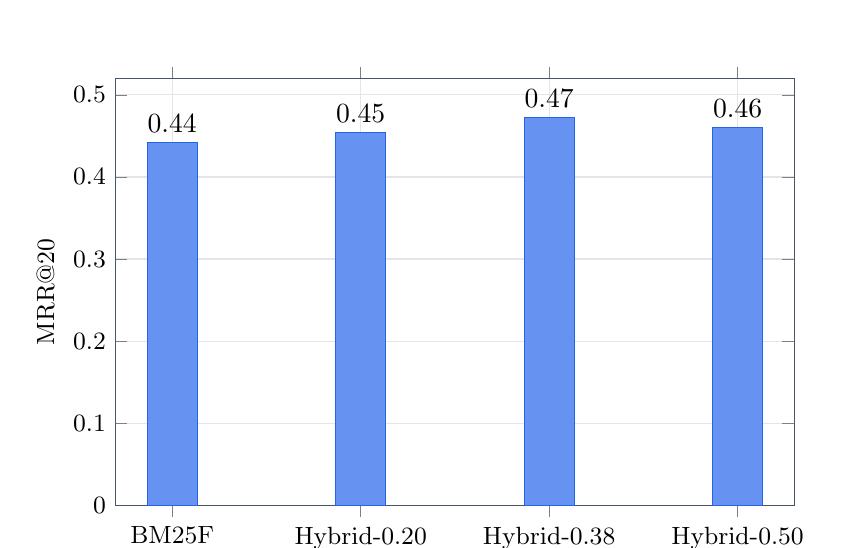
\begin{tikzpicture}
\begin{axis}[
  ybar,
  width=0.84\textwidth,
  height=7cm,
  ymin=0,ymax=0.52,
  ylabel={MRR@20},
  symbolic x coords={BM25F,Hybrid-0.20,Hybrid-0.38,Hybrid-0.50},
  xtick=data,
  nodes near coords,
  nodes near coords align={vertical},
  bar width=18pt,
  axis line style={draw=zetagray},
  tick label style={font=\small},
  label style={font=\small},
  grid=major,
  grid style={draw=zetagray!15}
]
\addplot[fill=zetablue!70,draw=zetablue] coordinates {
  (BM25F,0.4420) (Hybrid-0.20,0.4541) (Hybrid-0.38,0.4726) (Hybrid-0.50,0.4602)
};
\end{axis}
\end{tikzpicture}
\caption{BM25F 与不同 Hybrid 配置在 72 条查询上的 MRR@20}
\label{fig:mrr-comparison}
\end{figure}

其中，$\alpha=0.38$ 的 MRR@20 最高，比 BM25F 相对提高约 6.9\%。Top-1 则只多命中一条查询。结合不变的 Recall@20，这组结果支持在当前查询集上采用混合排名，改善主要体现在相关结果的排名上。

\subsection{混合系数消融}

融合系数增大，Dense 的权重就会上升，但排名未必继续改善。在 20 条查询上细化扫描步长后，$\alpha=0.37\sim0.39$ 均取得最高 MRR@20，值为 0.8896。

在另一组 72 条查询中，$\alpha=0.38$ 同样优于所比较的其他配置；增至 0.50 后，MRR@20 从 0.4726 降到 0.4602（图\ref{fig:alpha-ablation}）。两组查询不同，应各自在组内比较。

\begin{figure}[H]
\centering
\begin{tikzpicture}
\begin{axis}[
  width=0.84\textwidth,
  height=7cm,
  xlabel={Dense 融合系数 $\alpha$},
  ylabel={MRR@20},
  xmin=0.17,xmax=0.53,
  ymin=0.44,ymax=0.48,
  xtick={0.20,0.38,0.50},
  grid=both,
  grid style={draw=zetagray!15},
  tick label style={font=\small},
  label style={font=\small}
]
\addplot[color=zetagreen,mark=*,very thick] coordinates {
  (0.20,0.4541) (0.38,0.4726) (0.50,0.4602)
};
\end{axis}
\end{tikzpicture}
\caption{72 条查询上的固定混合系数消融}
\label{fig:alpha-ablation}
\end{figure}

据此，建议该查询集使用 $\alpha=0.38$；复现时显式传入该值，覆盖默认值 0.23。

\subsection{RAG 验证与单元测试}

检索排名不能代替答案检查。RAG 评测还需核对回答要点、完整集合计数和跨组证据。\path{evaluation/runner.py} 连接外部评测服务，仓库 \path{eval/} 下的脚本组织目标问题、随机查询及逐题调试输出。目标案例通过正则表达式检查答案要点；调试轨迹记录了 \code{collection}、\code{calculate} 的执行过程，以及 Verifier 审查后对答案所作的修订。

除逐题评测外，项目还用单元测试检查模块行为。历史记录显示，运行 \code{uv run python -m unittest discover -s tests} 后，132 项测试全部通过。测试范围包括：
\begin{itemize}
  \item 采集与存储：域名校验、重定向、断点恢复、正文提取和事务更新；
  \item 索引与检索：分块重叠、向量校验、原子 manifest、BM25F、Hybrid 和 reranker 高分平台；
  \item 问答：结构证据、完整表格、计算来源、多轮补检、答案槽位与一致性处理；
  \item 接口：HTTP 参数。
\end{itemize}

\section{应用与部署}

部署顺序是配置站点、采集网页、构建索引，再校准检索参数并接入 Web。RAG 上线前还应检查目标问题的调试输出：相关表格是否取全、计算用了哪些条目、最终引用是否对应答案。

查通知和师资信息时，搜索结果可直接引导用户回到网页。政策解释或办事流程适合使用 RAG，用户可通过答案中的引用核对原文。统计名单时，还可根据计算记录查阅所用的表格证据。

\section{结论}

本项目在检索与作答之间保留了一步原文恢复。索引使用固定分块，便于编码和排名；问答程序再从原文恢复完整结构，用于处理表格和名单。模型负责选择动作，程序负责执行数值运算，并为答案和计算结果保留来源引用。

现有评测中，$\alpha=0.38$ 是 72 条查询上表现最好的已测混合系数，复现这组结果时应显式指定。若更换站点或查询集，则应重新比较排名；默认值 0.23 与本组最优值不同，因此应针对实际查询集选择参数。

\printbibliography[title={参考文献}]

\appendix
\section{复现实验与代码阅读顺序}

\subsection{推荐复现步骤}

\begin{lstlisting}[language=bash,caption={测试与评测命令}]
uv sync
uv run python -m unittest discover -s tests
uv run zeta-engine eval --mode search --ranking hybrid --device cpu
uv run zeta-engine eval --mode rag --top-k 8 --device cpu
\end{lstlisting}

远端评测需配置服务和登录参数。已有评测数据见 \path{outputs/day5_high_confidence_mrr.json}、\path{outputs/hybrid_alpha_sweep.json} 和 \path{outputs/adapted_alpha_ablation_72.json}。

\subsection{推荐代码阅读顺序}

以下路径相对于 \path{src/zeta_engine/}，按数据进入系统到对外服务的顺序排列：

\begin{enumerate}
  \item \path{infrastructure/constants.py}、\path{ingestion/extraction_rules.py}、\path{ingestion/crawler.py}：采集范围、站点规则与抓取调度；
  \item \path{infrastructure/storage.py}、\path{infrastructure/tokenizer.py}：数据库访问、规范化与分词；
  \item \path{retrieval/index.py}、\path{retrieval/dense.py}、\path{retrieval/search.py}：倒排索引、共享 Passage、召回与重排；
  \item \path{retrieval/acquisition.py}：从候选 Passage 恢复语义结构，扫描完整表格；
  \item \path{application/service.py}：组织文档结果、获取证据，并向 RAG 注入工具；
  \item \path{rag/evidence.py}、\path{rag/protocol.py}、\path{rag/calculations.py}：证据池、动作校验与计算；
  \item \path{rag/engine.py}、\path{rag/__init__.py}，以及 \path{rag/prompts.py}、\path{rag/config.py}、\path{rag/types.py}：循环、入口、提示词、预算与返回结构；
  \item \path{interfaces/cli.py}、\path{interfaces/web.py}、\path{evaluation/runner.py}：用户接口与评测接入。
\end{enumerate}

\end{document}
